\section{Golub--Kahan双对角化}
\label{sec:ls-bidiagonal-iteration}

第~\ref{sec:ls-arnoldi}节的Arnoldi正交化与第~\ref{sec:ls-lanczos}节的Lanczos过程都针对方阵：残差与未知量同在$d$维空间，可以把残差反复乘$\bm A$。长方或秩亏的最小二乘问题中，$\bm A\in\mathbb R^{m\times d}$的残差在$m$维的数据空间，未知量在$d$维空间，不能把残差反复乘$\bm A$；把数据空间的向量送回未知量空间的是$\bm A^\top$。

这时需要的是第~\ref{sec:ls-krylov-subspaces}节所说的Krylov空间$\mathcal K_k(\bm A^\top\bm A,\bm A^\top\bm b)$。$\bm A^\top\bm A$对称半正定，原则上可以对它作Lanczos过程，但形成$\bm A^\top\bm A$会损失信息。\term{Golub--Kahan双对角化}（Golub--Kahan bidiagonalization）交替作用$\bm A$与$\bm A^\top$，只用$\bm A\bm v$与$\bm A^\top\bm u$，就得到与对$\bm A^\top\bm A$作Lanczos过程相同的基，并把$\bm A$压缩成一个双对角小矩阵。下面先推出两项递推，再写出计算过程，然后分析所得结果，最后说明它怎样用于求解最小二乘问题。

\subsection{主要思想}

给定$\bm A\in\mathbb R^{m\times d}$（可以秩亏）、$\bm b\in\mathbb R^m$与步数$k$，取零初值，初始残差就是$\bm b$。双对角化要在数据空间生成标准正交基$\bm u_1,\ldots,\bm u_{k+1}$，在未知量空间生成与之配对的标准正交基$\bm v_1,\ldots,\bm v_k$，使前$j$个$\bm v$张成$\mathcal K_j(\bm A^\top\bm A,\bm A^\top\bm b)$。第一对向量取$\bm u_1=\bm b/\lVert\bm b\rVert_2$，$\bm v_1$取$\bm A^\top\bm u_1$的方向。两组向量属于不同的空间，各自在本空间内正交。

\paragraph{交替的两项递推}
仿照第~\ref{sec:ls-arnoldi}节，新向量都由“乘矩阵、扣除旧基向量的分量、归一化”得到，只是$\bm A$与$\bm A^\top$交替使用：$\bm u_{j+1}$由$\bm A\bm v_j$对$\bm u_1,\ldots,\bm u_j$正交化得到，$\bm v_{j+1}$由$\bm A^\top\bm u_{j+1}$对$\bm v_1,\ldots,\bm v_j$正交化得到。

设此前的基已分别标准正交。按构造，每个$\bm A^\top\bm u_i$都是$\bm v_1,\ldots,\bm v_i$的组合，每个$\bm A\bm v_i$都是$\bm u_1,\ldots,\bm u_{i+1}$的组合。

于是$\bm A\bm v_j$在$\bm u_i$上的系数为
\[
 \bm u_i^\top\bm A\bm v_j=(\bm A^\top\bm u_i)^\top\bm v_j ,
\]
当$i<j$时$\bm A^\top\bm u_i$所含的$\bm v_1,\ldots,\bm v_i$都与$\bm v_j$正交，系数为零，只剩$i=j$一项。

同样，$\bm A^\top\bm u_{j+1}$在$\bm v_i$上的系数为
\[
 \bm v_i^\top\bm A^\top\bm u_{j+1}=(\bm A\bm v_i)^\top\bm u_{j+1} ,
\]
当$i<j$时$\bm A\bm v_i$所含的$\bm u_1,\ldots,\bm u_{i+1}$都与$\bm u_{j+1}$正交，系数为零，只剩$i=j$一项。

所以每生成一个新向量只需扣除对面空间中相邻的一个方向。把扣除的系数与归一化系数记为$\alpha_i,\beta_i\ge0$，并约定$\bm v_0=\bm 0$，列关系为
\begin{equation}
 \bm A\bm v_i=\alpha_i\bm u_i+\beta_{i+1}\bm u_{i+1},\qquad
 \bm A^\top\bm u_i=\beta_i\bm v_{i-1}+\alpha_i\bm v_i .
 \label{eq:ls-golub-kahan-columns}
\end{equation}

由第二式，$\bm A\bm v_j$在$\bm u_j$上的系数$(\bm A^\top\bm u_j)^\top\bm v_j$正是$\alpha_j$；由第一式，$\bm A^\top\bm u_{j+1}$在$\bm v_j$上的系数$(\bm A\bm v_j)^\top\bm u_{j+1}$正是$\beta_{j+1}$。因此扣除用的系数就是上一步的归一化系数，不必另作内积。

与Arnoldi正交化的列关系~\eqref{eq:ls-arnoldi-column}相比，每个像只用到对面空间中的两个基向量，不必保存整组基；这与Lanczos过程只需三项的原因相同，算法分析中将看到，右侧基正是$\bm A^\top\bm A$的Lanczos基。

\subsection{计算过程}

由列关系~\eqref{eq:ls-golub-kahan-columns}移项，每轮先作一次$\bm A$乘向量、扣除一个方向并归一化，得到新的$\bm u$，再作一次$\bm A^\top$乘向量、扣除一个方向并归一化，得到新的$\bm v$。下面写出计算中用到的变量、它们怎样初始化、每轮怎样更新。下面用以下不相容的长方系统逐步演示：
\[
 \bm A=\begin{bmatrix}1&0\\0&2\\0&0\end{bmatrix},\qquad
 \bm b=\begin{bmatrix}1\\1\\1\end{bmatrix}.
\]
第三行恒为零，$\bm b$的第三个分量无法拟合；最小二乘解是$\hat{\bm x}=(1,1/2)^\top$，最优残差为$(0,0,1)^\top$。这个例子的系数都有封闭形式，第~\ref{sec:ls-lsqr}节的LSQR与第~\ref{sec:ls-lsmr}节的LSMR继续用它，以便对照。

\paragraph{变量}
\begin{itemize}
 \item $\bm u_j\in\mathbb R^m$、$\bm v_j\in\mathbb R^d$：当前的两个基向量，只保存这两个；是否保存整组基由调用者决定。
 \item $\bm p\in\mathbb R^m$、$\bm q\in\mathbb R^d$：工作向量，分别存放数据空间与未知量空间中扣除后的余项。
 \item $\alpha_j$：$\bm B_k$的第$j$个对角元，也是$\bm v_j$的归一化系数。
 \item $\beta_j$：$\bm B_k$的第$j-1$列的次对角元（$\beta_1$为$\lVert\bm b\rVert_2$），也是$\bm u_j$的归一化系数。
 \item $j$：轮次。
\end{itemize}

\paragraph{初始化}
把$\bm u_1$初始化为$\bm b$的方向，再由列关系~\eqref{eq:ls-golub-kahan-columns}第二式在$i=1$时的$\bm A^\top\bm u_1=\alpha_1\bm v_1$把$\bm v_1$初始化为$\bm A^\top\bm u_1$的方向，轮次初始化为$1$：
\begin{equation}
 \begin{gathered}
 \beta_1=\lVert\bm b\rVert_2,\qquad \bm u_1=\frac{\bm b}{\beta_1},\\
 \alpha_1=\lVert\bm A^\top\bm u_1\rVert_2,\qquad \bm v_1=\frac{\bm A^\top\bm u_1}{\alpha_1}.
 \end{gathered}
 \label{eq:ls-golub-kahan-start}
\end{equation}
于是$\bm b=\beta_1\bm u_1$，而$\bm v_1$与$\bm A^\top\bm b$同向。

若$\bm b=\bm 0$，零向量满足方程；若$\alpha_1=0$，则$\bm A^\top\bm b=\bm 0$，零向量已满足正规方程~\eqref{eq:linear-algebra-normal-equations}。这两种情形都由求解器直接输出零向量，不再迭代。

例中$\beta_1=\sqrt3$，
\[
 \bm u_1=\frac1{\sqrt3}\begin{bmatrix}1\\1\\1\end{bmatrix},\qquad
 \bm A^\top\bm u_1=\frac1{\sqrt3}\begin{bmatrix}1\\2\end{bmatrix},
\]
故
\[
 \alpha_1=\sqrt{\frac53},\qquad \bm v_1=\frac{1}{\sqrt5}\begin{bmatrix}1\\2\end{bmatrix}.
\]

\paragraph{每轮更新}
在第$j$轮：
\begin{enumerate}
 \item \textbf{送到数据空间并扣除。}由列关系第一式（取$i=j$）移项，计算
 \[
  \bm p=\bm A\bm v_j-\alpha_j\bm u_j .
 \]
 例中第一轮
 \[
  \bm A\bm v_1=(1,4,0)^\top/\sqrt5,\qquad \alpha_1\bm u_1=\sqrt5(1,1,1)^\top/3 ,
 \]
 相减得
 \[
  \bm p=\frac{1}{3\sqrt5}\begin{bmatrix}-2\\7\\-5\end{bmatrix}.
 \]

 \item \textbf{归一化得到$\bm u_{j+1}$。}计算
 \[
  \beta_{j+1}=\lVert\bm p\rVert_2,\qquad \bm u_{j+1}=\frac{\bm p}{\beta_{j+1}} .
 \]
 例中第一轮
 \[
  \beta_2=\frac{\sqrt{78}}{3\sqrt5}\approx1.3166,\qquad
  \bm u_2=\frac{1}{\sqrt{78}}\begin{bmatrix}-2\\7\\-5\end{bmatrix}.
 \]

 \item \textbf{送回未知量空间并扣除。}由列关系第二式（取$i=j+1$）移项，计算
 \[
  \bm q=\bm A^\top\bm u_{j+1}-\beta_{j+1}\bm v_j .
 \]
 例中第一轮
 \[
  \bm A^\top\bm u_2=(-2,14)^\top/\sqrt{78},\qquad \beta_2\bm v_1=\sqrt{78}(1,2)^\top/15 ,
 \]
 相减得
 \[
  \bm q=\frac{18}{5\sqrt{78}}\begin{bmatrix}-2\\1\end{bmatrix}.
 \]

 \item \textbf{归一化得到$\bm v_{j+1}$。}计算
 \[
  \alpha_{j+1}=\lVert\bm q\rVert_2,\qquad \bm v_{j+1}=\frac{\bm q}{\alpha_{j+1}} .
 \]
 例中第一轮
 \[
  \alpha_2=\frac{18\sqrt5}{5\sqrt{78}}\approx0.9115,\qquad
  \bm v_2=\frac{1}{\sqrt5}\begin{bmatrix}-2\\1\end{bmatrix}.
 \]
 然后把本轮的$\beta_{j+1},\alpha_{j+1}$及新基向量交给调用它的求解器，令$j\leftarrow j+1$。

 例中第二轮
 \[
  \bm p=\bm A\bm v_2-\alpha_2\bm u_2=\frac{5}{13\sqrt5}\begin{bmatrix}-4\\1\\3\end{bmatrix},
 \]
 归一化得
 \[
  \beta_3=\sqrt{\frac{10}{13}}\approx0.8771,\qquad
  \bm u_3=\frac1{\sqrt{26}}\begin{bmatrix}-4\\1\\3\end{bmatrix};
 \]
 再送回未知量空间，
 \[
  \bm A^\top\bm u_3=(-4,2)^\top/\sqrt{26}
 \]
 恰好等于$\beta_3\bm v_2$，所以
 \[
  \bm q=\bm 0,\qquad \alpha_3=0 .
 \]

 \item \textbf{停止。}若$\beta_{j+1}=0$（实际中低于按数据尺度取定的阈值），则$\bm A\bm v_j=\alpha_j\bm u_j$，不生成$\bm u_{j+1}$，约定$\alpha_{j+1}=0$并退出迭代；若$\beta_{j+1}>0$而$\alpha_{j+1}=0$，则$\bm A^\top\bm u_{j+1}=\beta_{j+1}\bm v_j$已由现有的基表示，不生成$\bm v_{j+1}$，退出迭代；否则在求解器决定继续时进入下一轮，至多做满$k$轮。
 
 两种情况下略去未生成的基向量及其零系数，列关系~\eqref{eq:ls-golub-kahan-columns}仍成立；求解器照常用本轮的系数完成解的更新后再结束。基停止扩张不等于原残差为零：不相容问题的原残差可以停在非零值上。
 
 例中第二轮$\alpha_3=0$，未知量空间只有二维，已被$\bm v_1,\bm v_2$取尽，退出迭代。
\end{enumerate}
第1—4步合起来就是
\begin{equation}
 \begin{aligned}
 \bm p&=\bm A\bm v_j-\alpha_j\bm u_j, & \beta_{j+1}&=\lVert\bm p\rVert_2, & \bm u_{j+1}&=\bm p/\beta_{j+1},\\
 \bm q&=\bm A^\top\bm u_{j+1}-\beta_{j+1}\bm v_j, & \alpha_{j+1}&=\lVert\bm q\rVert_2, & \bm v_{j+1}&=\bm q/\alpha_{j+1} .
 \end{aligned}
 \label{eq:ls-golub-kahan-step}
\end{equation}

最终得到两组标准正交基与各轮系数组成的下双对角矩阵。例中$\bm U_3=[\bm u_1\;\bm u_2\;\bm u_3]$，
\[
 \bm V_2=\frac1{\sqrt5}\begin{bmatrix}1&-2\\2&1\end{bmatrix},\qquad
 \bm B_2=\begin{bmatrix}\alpha_1&0\\\beta_2&\alpha_2\\0&\beta_3\end{bmatrix}
 \approx\begin{bmatrix}1.2910&0\\1.3166&0.9115\\0&0.8771\end{bmatrix},
\]
它们满足
\[
 \bm A\bm V_2=\bm U_3\bm B_2 .
\]
逐列核对：
\[
 \begin{gathered}
 \alpha_1\bm u_1+\beta_2\bm u_2=(1,4,0)^\top/\sqrt5=\bm A\bm v_1,\\
 \alpha_2\bm u_2+\beta_3\bm u_3=(-2,2,0)^\top/\sqrt5=\bm A\bm v_2 .
 \end{gathered}
\]
右侧二维空间已经生成完毕，但$\bm b$的第三个分量仍不可拟合，原残差不会降到零。

上面的例子中基向量都有简单的封闭形式。对稠密的矩阵，可以只用双对角系数本身来核对计算，下面在直线拟合上演示。

\begin{example}[直线拟合上的两步双对角化]
\label{ex:ls-golub-kahan-line}
沿用示例~\ref{ex:ls-line-least-squares}的数据：
\[
 \bm A=\begin{bmatrix}1&0\\1&1\\1&2\end{bmatrix},\qquad
 \bm b=\begin{bmatrix}1\\2\\2\end{bmatrix}.
\]
起步得
\[
 \beta_1=3,\qquad \bm u_1=(1,2,2)^\top/3 ;
\]
再由$\bm A^\top\bm u_1=(5/3,2)^\top$得
\[
 \alpha_1=\sqrt{61}/3\approx2.6034,\qquad \bm v_1=(5,6)^\top/\sqrt{61} .
\]

第一轮先把$\bm v_1$送到数据空间并扣除$\alpha_1\bm u_1$：
\[
 \begin{gathered}
 \bm A\bm v_1=\frac{(5,11,17)^\top}{\sqrt{61}},\\
 \bm p=\bm A\bm v_1-\alpha_1\bm u_1=\frac{(-16,-23,31)^\top}{9\sqrt{61}},
 \end{gathered}
\]
于是
\[
  \beta_2\approx0.5944, \qquad \bm u_2\approx(-0.3829,-0.5504,0.7419)^\top .
\]
再由$\bm A^\top\bm u_2-\beta_2\bm v_1$得
\[
  \alpha_2\approx0.7446, \qquad \bm v_2=(-6,5)^\top/\sqrt{61} .
\]

第二轮得
\[
  \beta_3\approx0.5607, \qquad \bm u_3\approx(-0.8615,0.5026,-0.0718)^\top ,
\]
而$\bm A^\top\bm u_3-\beta_3\bm v_2=\bm0$，即$\alpha_3=0$：未知量空间只有二维，已被$\bm v_1,\bm v_2$取尽，生成到此为止。

最后核对结果。$\bm u_1,\bm u_2,\bm u_3$两两正交；$\bm V_2$是正交方阵，$\bm A=\bm U_3\bm B_2\bm V_2^\top$，所以$\bm B_2^\top\bm B_2$与$\bm A^\top\bm A=\left[\begin{smallmatrix}3&3\\3&5\end{smallmatrix}\right]$有相同的迹$8$和行列式$6$。数值上
\[
 \begin{gathered}
 \alpha_1^2+\beta_2^2+\alpha_2^2+\beta_3^2\approx8.000,\\
 \alpha_1^2\alpha_2^2+\alpha_1^2\beta_3^2+\beta_2^2\beta_3^2\approx6.000 .
 \end{gathered}
\]
两个不变量都吻合。这项核对只用到双对角系数本身，不必重新比较各个基向量。
\end{example}

\subsection{算法分析}

\paragraph{基矩阵与投影矩阵}
把各步得到的两组基分别并排，记
\begin{equation}
 \bm U_{k+1}=[\bm u_1\;\cdots\;\bm u_{k+1}]\in\mathbb R^{m\times(k+1)},\qquad
 \bm V_k=[\bm v_1\;\cdots\;\bm v_k]\in\mathbb R^{d\times k},
 \label{eq:ls-golub-kahan-bases}
\end{equation}
两者通常都是瘦长矩阵。

把$i=1,\ldots,k$的第一式与$i=1,\ldots,k+1$的第二式分别并排写出，得到
\begin{equation}
 \bm A\bm V_k=\bm U_{k+1}\bm B_k,\qquad
 \bm A^\top\bm U_{k+1}=\bm V_k\bm B_k^\top+\alpha_{k+1}\bm v_{k+1}\bm e_{k+1}^\top ,
 \label{eq:ls-golub-kahan-relations}
\end{equation}
其中
\begin{equation}
 \bm B_k=
 \begin{bmatrix}
 \alpha_1&&&\\
 \beta_2&\alpha_2&&\\
 &\beta_3&\ddots&\\
 &&\ddots&\alpha_k\\
 &&&\beta_{k+1}
 \end{bmatrix}
 \label{eq:ls-golub-kahan-bidiagonal-matrix}
\end{equation}
是$(k+1)\times k$的下双对角矩阵，第$i$列只有$\alpha_i$和它下方的$\beta_{i+1}$。后一式的边界项来自$\bm u_{k+1}$被$\bm A^\top$送回时产生的新方向；$\alpha_{k+1}=0$时它为零。

第一式左乘$\bm U_{k+1}^\top$，并用$\bm U_{k+1}^\top\bm U_{k+1}=\bm I$，得
\begin{equation}
 \bm B_k=\bm U_{k+1}^\top\bm A\bm V_k .
 \label{eq:ls-golub-kahan-projection}
\end{equation}
所以$\bm B_k$是$\bm A$从$\operatorname{range}(\bm V_k)$到$\operatorname{range}(\bm U_{k+1})$的坐标矩阵：若$\bm z=\bm V_k\bm y$，则$\bm A\bm z=\bm U_{k+1}\bm B_k\bm y$完全落在$\operatorname{range}(\bm U_{k+1})$中，坐标为$\bm B_k\bm y$。$m\times d$的长方矩阵就这样被压缩成一个$(k+1)\times k$的下双对角矩阵，只需$2k$个数记录。

再由第一式，
\begin{equation}
 \bm V_k^\top\bm A^\top\bm A\bm V_k=\bm B_k^\top\bm U_{k+1}^\top\bm U_{k+1}\bm B_k=\bm B_k^\top\bm B_k ,
 \label{eq:ls-golub-kahan-normal-projection}
\end{equation}
$\bm B_k^\top\bm B_k$是对称三对角矩阵，对角元为$\alpha_i^2+\beta_{i+1}^2$，次对角元为$\alpha_{i+1}\beta_{i+1}$；它就是对称半正定矩阵$\bm A^\top\bm A$在$\operatorname{range}(\bm V_k)$上的投影，相当于对$\bm A^\top\bm A$作Lanczos过程得到的$\bm T_k$。

\paragraph{正确性}
上面的论证用到了两组基的标准正交性，而每步只扣除一项。下面的定理说明，短递推~\eqref{eq:ls-golub-kahan-step}得到的两组基确实标准正交，关系~\eqref{eq:ls-golub-kahan-relations}成立，并且右侧基张成正规方程的Krylov空间。

\begin{theorem}[Golub--Kahan关系]
\label{thm:ls-golub-kahan-relations}
设$\alpha_1,\ldots,\alpha_k$与$\beta_2,\ldots,\beta_{k+1}$都为正。则在精确算术中，$\bm U_{k+1}$与$\bm V_k$的列分别标准正交，关系~\eqref{eq:ls-golub-kahan-relations}成立，其中$\alpha_{k+1}=0$时末项为零；并且$\operatorname{range}(\bm V_k)=\mathcal K_k(\bm A^\top\bm A,\bm A^\top\bm b)$。
\end{theorem}

\begin{proof}
先说明矩阵关系只是列关系的汇总，再对轮数归纳证明正交性，最后确定右侧基张成的空间。

\emph{列关系。}由式~\eqref{eq:ls-golub-kahan-start}与\eqref{eq:ls-golub-kahan-step}中$\bm p,\bm q$的定义，列关系~\eqref{eq:ls-golub-kahan-columns}成立。$\bm B_k^\top$的第$i$列是$\bm B_k$的第$i$行，所以它们分别是式~\eqref{eq:ls-golub-kahan-relations}两式的第$i$列；第二式第$k+1$列中$\alpha_{k+1}\bm v_{k+1}$一项不在$\bm V_k$中，单独写成边界项。

\emph{正交性。}设$\bm u_1,\ldots,\bm u_k$与$\bm v_1,\ldots,\bm v_k$已分别标准正交。对$j\le k$，由列关系，
\[
 \begin{aligned}
 \beta_{k+1}\bm u_j^\top\bm u_{k+1}
 &=\bm v_k^\top\bm A^\top\bm u_j-\alpha_k\bm u_j^\top\bm u_k\\
 &=\bm v_k^\top(\beta_j\bm v_{j-1}+\alpha_j\bm v_j)-\alpha_k\delta_{j,k}=0 .
 \end{aligned}
\]
再由$\bm A\bm v_j=\alpha_j\bm u_j+\beta_{j+1}\bm u_{j+1}$以及刚证明的$\bm u$的正交性，
\[
 \alpha_{k+1}\bm v_j^\top\bm v_{k+1}=\bm u_{k+1}^\top\bm A\bm v_j-\beta_{k+1}\delta_{j,k}=\beta_{j+1}\delta_{j,k}-\beta_{k+1}\delta_{j,k}=0 .
\]

\emph{张成的空间。}$\bm v_1\parallel\bm A^\top\bm b$；把两条列关系代入$\bm A^\top\bm A\bm v_i$，得
\[
 \alpha_{i+1}\beta_{i+1}\bm v_{i+1}=\bm A^\top\bm A\bm v_i-(\alpha_i^2+\beta_{i+1}^2)\bm v_i-\alpha_i\beta_i\bm v_{i-1},
\]
归纳可知$\bm v_i\in\mathcal K_i(\bm A^\top\bm A,\bm A^\top\bm b)$。$\bm V_k$的$k$列标准正交，而该Krylov空间至多$k$维，两者相等。
\end{proof}

因此零初值下双对角化生成的正是第~\ref{sec:ls-krylov-subspaces}节所说的长方矩阵Krylov空间，但从不形成$\bm A^\top\bm A$。证明中的三项关系就是对$\bm A^\top\bm A$从$\bm A^\top\bm b$出发的Lanczos递推~\eqref{eq:ls-arnoldi-lanczos}，其中$a_i=\alpha_i^2+\beta_{i+1}^2$、$\gamma_i=\alpha_{i+1}\beta_{i+1}$，正是$\bm B_k^\top\bm B_k$的元素。图~\ref{fig:ls-golub-kahan-bidiagonal}把递推与矩阵关系放在一起：(a)中进出$\bm v_i$的两支箭头给出$\alpha_i$与$\beta_{i+1}$，它们正是(b)中$\bm B_k$的第$i$列；每个新向量只与对面空间中相邻的一个向量相连，这就是每步只需扣除一项的原因。

\begin{figure}[htbp]
  \centering
  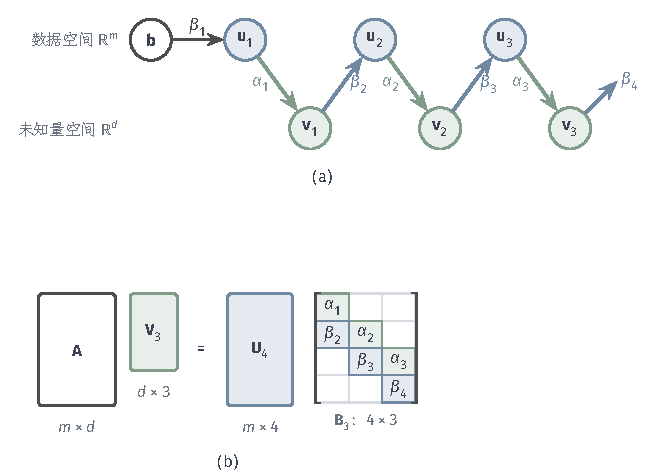
\includegraphics[width=109.343mm]{figures/01-basic-mathematics/03-vectors-matrices-and-multivariate-functions/tikz/c5-golub-kahan-bidiagonal/figure.pdf}
  \caption{Golub--Kahan双对角化的递推与矩阵关系（$k=3$）。(a)蓝色$\bm u_i$在数据空间，绿色$\bm v_i$在未知量空间；乘$\bm A^\top$并扣除前一个$\bm v$后归一化得到$\bm v_i$，长度为$\alpha_i$，乘$\bm A$并扣除前一个$\bm u$后归一化得到$\bm u_{i+1}$，长度为$\beta_{i+1}$。(b)这些长度排成$4\times3$的下双对角矩阵$\bm B_3$，满足$\bm A\bm V_3=\bm U_4\bm B_3$；绿格为对角元，蓝格为次对角元，其余元素为零。}
  \label{fig:ls-golub-kahan-bidiagonal}
\end{figure}

\paragraph{数值敏感度}
在浮点运算中，正交性所依赖的相消只近似成立，短递推也不会去掉舍入引入的旧方向分量，两组基会逐渐失去正交性；它对求解结果的影响交给两种求解器，由求解器在停止前的真实残差复核来控制，必要时以保存基并重正交化的代价换取正交性。

\paragraph{计算代价}
每轮至多一次$\bm A$乘向量和一次$\bm A^\top$乘向量，外加两次向量更新、两次范数和两次缩放。调用者只用当前的$\bm u_k,\bm v_k$，不保存整组基、不作完整再正交化时，工作存储为$O(m+d)$，与Lanczos过程一样不随轮数增长。双对角化只负责生成候选空间，收敛快慢取决于求解器在子空间中怎样选取近似解。

\subsection{应用}
\label{sec:ls-golub-kahan-application}

有了两组基与双对角矩阵，就可以在子空间中求解最小二乘问题。零初值下把近似写成
\[
 \bm x=\bm V_k\bm y ,
\]
$\bm y\in\mathbb R^k$是$\mathcal K_k(\bm A^\top\bm A,\bm A^\top\bm b)$中的坐标。

由$\bm b=\beta_1\bm u_1=\bm U_{k+1}\beta_1\bm e_1$与关系~\eqref{eq:ls-golub-kahan-relations}的第一式，
\begin{equation}
 \bm b-\bm A\bm V_k\bm y=\bm U_{k+1}\bigl(\beta_1\bm e_1-\bm B_k\bm y\bigr).
 \label{eq:ls-golub-kahan-residual-coordinates}
\end{equation}
$\bm U_{k+1}$的列标准正交，不改变长度，所以在子空间中使原残差最小，化为$(k+1)\times k$的双对角最小二乘问题
\begin{equation}
 \min_{\bm y}\lVert\beta_1\bm e_1-\bm B_k\bm y\rVert_2 .
 \label{eq:ls-golub-kahan-lsqr-problem}
\end{equation}
这就是LSQR（第~\ref{sec:ls-lsqr}节）的做法；$\bm B_k$每增加一列只在右下角多出两个非零元，一次新的正交变换就能延续三角化，解可以由短递推逐步累加。

若改为使正规残差最小，再用关系~\eqref{eq:ls-golub-kahan-relations}的第二式把$\bm A^\top$作用上去。$\bm B_k$的首行是$\alpha_1\bm e_1^\top$、末行是$\beta_{k+1}\bm e_k^\top$，于是
\begin{equation}
 \bm A^\top\bigl(\bm b-\bm A\bm V_k\bm y\bigr)
 =\bm V_k\bigl(\alpha_1\beta_1\bm e_1-\bm B_k^\top\bm B_k\bm y\bigr)-\alpha_{k+1}\beta_{k+1}y_k\bm v_{k+1},
 \label{eq:ls-golub-kahan-normal-residual-coordinates}
\end{equation}
其中$y_k$是$\bm y$的末分量。右端仍由标准正交的$\bm v_1,\ldots,\bm v_{k+1}$表示，正规残差的长度因此也化为关于三对角矩阵$\bm B_k^\top\bm B_k$及一个边界项的小问题。这就是LSMR（第~\ref{sec:ls-lsmr}节）的做法，它实际计算时并不形成$\bm B_k^\top\bm B_k$。

两者的子空间、两组基和双对角矩阵都来自同一个双对角化，区别只在于最小化原残差还是正规残差。它们与方阵情形的对应也很清楚：对正规方程而言，LSQR相当于在Lanczos基上用Galerkin条件，LSMR相当于极小残差条件，第~\ref{sec:ls-lsqr}节与第~\ref{sec:ls-lsmr}节将分别证明它们与正规方程上的CG和MINRES等价。
